\documentclass{beamer}
\let\vec\mathbf
\mode<presentation>
\usepackage{amsmath}
\usepackage{amssymb}
%\usepackage{advdate}
\usepackage{adjustbox}
%\usepackage{subcaption}
%\usepackage{enumitem}
\usepackage{multicol}
\usepackage{mathtools}
\usepackage{tikz}
\usepackage{listings}
\usepackage{url}
\usetheme{Boadilla}
\usecolortheme{lily}
\setbeamertemplate{footline}
{
  \leavevmode%
  \hbox{%
  \begin{beamercolorbox}[wd=\paperwidth,ht=2.25ex,dp=1ex,right]{author in head/foot}%
    \insertframenumber{} / \inserttotalframenumber\hspace*{2ex}
  \end{beamercolorbox}}%
  \vskip0pt%
}
\setbeamertemplate{navigation symbols}{}
\providecommand{\nCr}[2]{\,^{#1}C_{#2}} % nCr
\providecommand{\nPr}[2]{\,^{#1}P_{#2}} % nPr
\providecommand{\mbf}{\mathbf}
\providecommand{\pr}[1]{\ensuremath{\Pr\left(#1\right)}}
\providecommand{\qfunc}[1]{\ensuremath{Q\left(#1\right)}}
\providecommand{\sbrak}[1]{\ensuremath{{}\left[#1\right]}}
\providecommand{\lsbrak}[1]{\ensuremath{{}\left[#1\right.}}
\providecommand{\rsbrak}[1]{\ensuremath{{}\left.#1\right]}}
\providecommand{\brak}[1]{\ensuremath{\left(#1\right)}}
\providecommand{\lbrak}[1]{\ensuremath{\left(#1\right.}}
\providecommand{\rbrak}[1]{\ensuremath{\left.#1\right)}}
\providecommand{\cbrak}[1]{\ensuremath{\left\{#1\right\}}}
\providecommand{\lcbrak}[1]{\ensuremath{\left\{#1\right.}}
\providecommand{\rcbrak}[1]{\ensuremath{\left.#1\right\}}}
\theoremstyle{remark}
\newtheorem{rem}{Remark}
\newcommand{\sgn}{\mathop{\mathrm{sgn}}}

\providecommand{\res}[1]{\Res\displaylimits_{#1}}
\providecommand{\norm}[1]{\lVert#1\rVert}
\providecommand{\mtx}[1]{\mathbf{#1}}

\providecommand{\fourier}{\overset{\mathcal{F}}{ \rightleftharpoons}}
%\providecommand{\hilbert}{\overset{\mathcal{H}}{ \rightleftharpoons}}
\providecommand{\system}{\overset{\mathcal{H}}{ \longleftrightarrow}}
    %\newcommand{\solution}[2]{\textbf{Solution:}{#1}}
%\newcommand{\solution}{\noindent \textbf{Solution: }}
\providecommand{\dec}[2]{\ensuremath{\overset{#1}{\underset{#2}{\gtrless}}}}
\newcommand{\myvec}[1]{\ensuremath{\begin{pmatrix}#1\end{pmatrix}}}

\title{Matrices in Geometry - 4.13.40}
\author{EE25BTECH11035 Kushal B N}
\date{Sep, 2025}

\begin{document}

\maketitle

\section{Problem Statement}
\begin{frame}{Problem Statement}

The number of integer values of $m$ for which the x-coordinate of the point of intersection of the lines $3x + 4y = 9$ and $y = mx + 1$ is also an integer, is
  \begin{enumerate}
    \item 2
    \item 0
    \item 4
    \item 1
  \end{enumerate}
\end{frame}

\section{Solution}
\begin{frame}{Solution}
Given,\\
The two lines\\
$\myvec{3&4}\myvec{x\\y}=9$ and $\myvec{m&-1}\myvec{x\\y}=-1$
The given set of equations can be written as,
\begin{equation}
    \myvec{3&4\\m&-1}\myvec{x\\y} = \myvec{9\\-1}
\end{equation}

Augmented Matrix:
\begin{equation}
    \myvec{3&4&|&9\\m&-1&|&-1}
\end{equation}

\begin{equation}
    \myvec{3&4&|&9\\m&-1&|&-1} \overset{R_2 \rightarrow R_2 - \frac{m}{3}R_1}{\longrightarrow} \myvec{3&4&|&9\\0&-1-\frac{4m}{3}&|&-1-3m}
\end{equation}

\begin{equation}
    \implies y = 3\brak{\frac{3m+1}{4m+3}}
\end{equation}
\end{frame}

\begin{frame}{Solution}
\begin{equation}
    \implies x = \frac{5}{4m+3}
\end{equation}
Thus, for $x$ to be an integer, while keeping the denominator also an integer,\\
\begin{equation}
\brak{4m+3} \in \cbrak{1,5,-1,-5}
\end{equation}

\begin{equation}
    \implies m \in \cbrak{\frac{-1}{2},\frac{1}{2},-1,-2}
\end{equation}

Hence, for m to be an integer value $m = -1$ or $m = -2$.
\end{frame}

\section{Conclusion}
\begin{frame}{Conclusion}
$\therefore$ There are 2 integer values of $m$ for which the x-coordinate of the point of intersection of the given lines is also an integer.\\
Hence, the correct answer is option (1).

\begin{figure}[H]
    \centering
    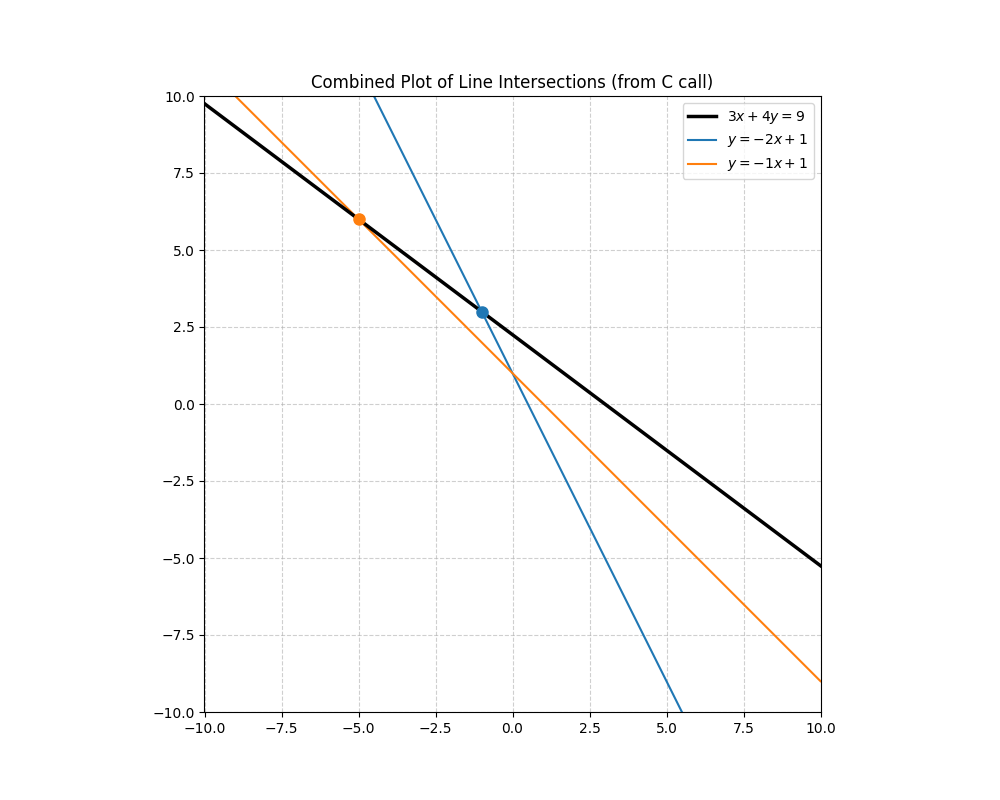
\includegraphics[width=0.65\columnwidth]{figs/1.png}
    \caption{}
\end{figure}

\end{frame}
\end{document}